\section{Theory} \label{sec:theory}
To calculate the energies, we need to solve the Schrödinger equation
\begin{equation}
\hat{H}\ket{\Psi_p}=\varepsilon_p\ket{\Psi_p}
\end{equation}
where we expect to find the exact ground state energy, $\varepsilon_0$, when the correct ground state wave function (GSWF) has been used. In this project we will stick to the Born-Oppenheimer approximation, which gives the Hamiltonian when the nucleus is stationary (is not affected by the electrons),
\begin{equation}
\hat{H}=\sum_{i=1}^Nt(x_i)-\sum_{i=1}^Nk\frac{Ze^2}{r_i}+\sum_{i<j}^N\frac{ke^2}{r_{ij}}.
\end{equation}
The first term gives the kinetic energy, the second gives the energy from the external potential (nucleus) and the last term gives the interaction energy. $Z$ is the atomic number, defining the number of protons in the nucleus, $k$ is the constant from Coulomb's law and $e$ is the elementary change.

We now introduce the atomic units, setting $\hbar=c=e=m_e=k=1$. 
The energies can be converted between atomic units and electronvolts using the relation
\begin{equation}
1 \text{ a.u.} = 2\cdot13.6 \text{ eV}.
\end{equation}
The Hamiltonian now reads
\begin{equation}
\hat{H}=\hat{H}_0 + \hat{H}_I=\sum_{i=1}^N\hat{h}_0(x_i)+\sum_{i<j}^N\frac{1}{r_{ij}}
\end{equation}
with $r_{ij}\equiv\frac{1}{|\boldsymbol{r}_i-\boldsymbol{r}_j|}$ and $\hat{h}_0$ as the one-body operator for each electron. The single particle functions (SPF) are assumed to be hydrogen-like, where the one-body energies are known from the Bohr model, stating
\begin{equation}
E_n=-\frac{Z^2}{2n^2}
\end{equation}
where $n$ is the number of nodes in the wave function. In order to calculate the two-body energies, we need to solve the integrals 
\begin{equation}
\int r_1^2dr_1\int r_2^2dr_2 \Phi_{\alpha}^*(r_1)\Phi_{\beta}^*(r_2)\frac{1}{|\boldsymbol{r}_1-\boldsymbol{r}_2|}\Phi_{\gamma}(r_1)\Phi_{\delta}(r_2)\equiv\mel{\alpha\beta}{\hat{v}}{\gamma\delta}
\end{equation}
where the Dirac notation is used for shorthand notation. Note carefully that the $\Phi$'s are the total wave functions, where both the radial and spin parts are included. The spin part is known to not affect the energies, and it can therefore be factorized out,
\begin{align}
\mel{\alpha\beta}{\hat{v}}{\gamma\delta}&=(\alpha\beta|\hat{v}|\gamma\delta)\braket{\chi_{\alpha}\chi_{\beta}}{\chi_{\gamma}\chi_{\delta}}\notag\\
&=(\alpha\beta|\hat{v}|\gamma\delta)\braket{\chi_{\alpha}}{\chi_{\gamma}}\braket{\chi_{\beta}}{\chi_{\delta}}\\
&=(\alpha\beta|\hat{v}|\gamma\delta)\,\delta_{\sigma_{\alpha}\sigma_{\gamma}}\delta_{\sigma_{\beta}\sigma_{\delta}}.\notag
\end{align}
We observe that the integral is non-zero if and only if $\alpha$ and $\gamma$ got the same spin, and $\beta$ and $\delta$ got the same spin.

For calculating the ground state energy of an atom with atomic number $Z$, we need to calculate
\begin{align}
\varepsilon_0=\mel{\Phi_0}{\hat{H}}{\Phi_0}&=\sum_i\mel{i}{\hat{h}_0}{i}+\frac{1}{2}\sum_{ij}\Big[\mel{ij}{\hat{v}}{ij}-\mel{ij}{\hat{v}}{ji}\Big]\\
&=E_0(Z)+\hdots
\end{align}
See appendix A. 

\subsection{Second Quantization}
Define the Hamiltonian in second quantization

\subsubsection{Wick's theorem}

Should also write about spins, Pauli principle, quantum numbers and so on. 


\subsection{The Helium atom}
A neutral Helium atom consists of a nucleus of two protons with two electrons swarming around it, and is one of the most simple many-body systems one can study. The difficulty of dealing with many-body systems lies in the interaction, where the elements $\mel{\alpha\beta}{\hat{v}}{\gamma\delta}$ can be really tricky to handle. Hard to find exact wave function. 

There exist various methods for solving this problem, where one of the most successful is to define a wave function which is varied such that the energy is minimized. This method was used by E. Hylleraas already in 1929, when he minimized the energy with a wave function of 10 variational parameters, using a mechanical desk calculator. [https://www.encyclopedia.com/science/dictionaries-thesauruses-pictures-and-press-releases/hylleraas-egil-andersen] He found the energy to be -2.90363 eV, which is close to recent experimental values. [http://www.umich.edu/~chem461/QMChap8.pdf][https://journals.aps.org/prl/abstract/10.1103/PhysRevLett.80.3475]. 




Lide 1992
Handbook of Chem. and Phys. lide 1992



\subsubsection{Ground state}
Spin up/spin down - Pauli principle - Slater determinant - Dirac notation
\begin{figure} [H]
	\begin{center}
		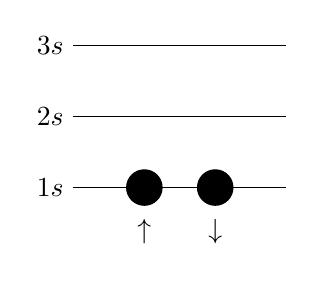
\begin{tikzpicture}[scale=0.9]
		\begin{scope}
			\foreach \i in {1,...,3}
			{
				\draw (-1,\i-1) node[anchor=east] {$\i s$} --(2,\i-1);
			}
			\filldraw (0,0) node[anchor=north,inner sep=.4cm] {$\uparrow$} circle (0.25cm); 
			\filldraw (1,0) node[anchor=north,inner sep=.4cm] {$\downarrow$} circle (0.25cm);
		\end{scope}
		\end{tikzpicture}
	\end{center}
\caption{}
\label{fig:schematic_he_gs}
\end{figure}

\subsubsection{Excited states}
Consider now a system consisting of the orbitals 1s, 2s and 3s only. For that case, the possible energy states of the Helium atom are listed in figure \eqref{fig:schematic_he}.
\begin{figure} [H]
	\begin{center}
		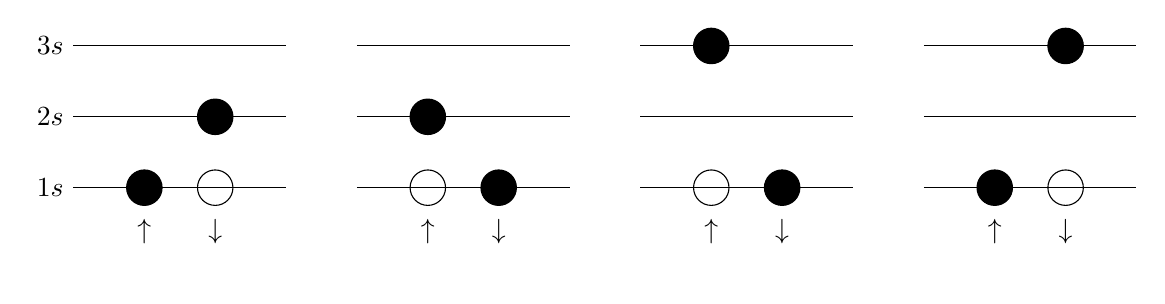
\begin{tikzpicture}[scale=0.9]
		\begin{scope}
		\foreach \i in {1,...,3}
		{
			\draw (-1,\i-1) node[anchor=east] {$\i s$} --(2,\i-1);
		}
		\filldraw (0,0) node[anchor=north,inner sep=.4cm] {$\uparrow$} circle (0.25cm); 
		\draw (1,0) node[anchor=north,inner sep=.4cm] {$\downarrow$} circle (0.25cm);
		\filldraw (1,1) circle (0.25cm);
		\end{scope}
		\begin{scope}[xshift=4cm]
		\foreach \i in {1,...,3}
		{
			\draw (-1,\i-1) --(2,\i-1);
		}
		\draw (0,0) node[anchor=north,inner sep=.4cm] {$\uparrow$} circle (0.25cm); 
		\filldraw (1,0) node[anchor=north,inner sep=.4cm] {$\downarrow$} circle (0.25cm);
		\filldraw (0,1) circle (0.25cm); 
		\end{scope}
		\begin{scope}[xshift=8cm]
		\foreach \i in {1,...,3}
		{
			\draw (-1,\i-1) --(2,\i-1);
		}
		\draw (0,0) node[anchor=north,inner sep=.4cm] {$\uparrow$} circle (0.25cm); 
		\filldraw (1,0) node[anchor=north,inner sep=.4cm] {$\downarrow$} circle (0.25cm);
		\filldraw (0,2) circle (0.25cm); 
		\end{scope}
		\begin{scope}[xshift=12cm]
		\foreach \i in {1,...,3}
		{
			\draw (-1,\i-1) --(2,\i-1);
		}
		\filldraw (0,0) node[anchor=north,inner sep=.4cm] {$\uparrow$} circle (0.25cm); 
		\draw (1,0) node[anchor=north,inner sep=.4cm] {$\downarrow$} circle (0.25cm);
		\filldraw (1,2) circle (0.25cm); 
		\end{scope}
		\end{tikzpicture}
		\newline
		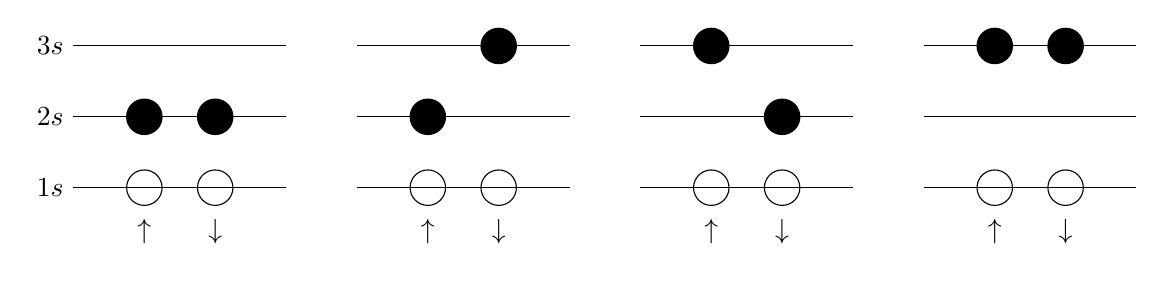
\begin{tikzpicture}[scale=0.9]
		\begin{scope}
		\foreach \i in {1,...,3}
		{
			\draw (-1,\i-1) node[anchor=east] {$\i s$} --(2,\i-1);
		}
		\draw (0,0) node[anchor=north,inner sep=.4cm] {$\uparrow$} circle (0.25cm); 
		\draw (1,0) node[anchor=north,inner sep=.4cm] {$\downarrow$} circle (0.25cm);
		\filldraw (0,1) circle (0.25cm);
		\filldraw (1,1) circle (0.25cm);
		\end{scope}
		\begin{scope}[xshift=4cm]
		\foreach \i in {1,...,3}
		{
			\draw (-1,\i-1) --(2,\i-1);
		}
		\draw (0,0) node[anchor=north,inner sep=.4cm] {$\uparrow$} circle (0.25cm); 
		\draw (1,0) node[anchor=north,inner sep=.4cm] {$\downarrow$} circle (0.25cm);
		\filldraw (1,2) circle (0.25cm);
		\filldraw (0,1) circle (0.25cm);
		\end{scope}
		\begin{scope}[xshift=8cm]
		\foreach \i in {1,...,3}
		{
			\draw (-1,\i-1) --(2,\i-1);
		}
		\draw (0,0) node[anchor=north,inner sep=.4cm] {$\uparrow$} circle (0.25cm); 
		\draw (1,0) node[anchor=north,inner sep=.4cm] {$\downarrow$} circle (0.25cm);
		\filldraw (0,2) circle (0.25cm); 
		\filldraw (1,1) circle (0.25cm); 
		\end{scope}
		\begin{scope}[xshift=12cm]
		\foreach \i in {1,...,3}
		{
			\draw (-1,\i-1) --(2,\i-1);
		}
		\draw (0,0) node[anchor=north,inner sep=.4cm] {$\uparrow$} circle (0.25cm); 
		\draw (1,0) node[anchor=north,inner sep=.4cm] {$\downarrow$} circle (0.25cm);
		\filldraw (0,2) circle (0.25cm); 
		\filldraw (1,2) circle (0.25cm);
		\end{scope}
		\end{tikzpicture}
	\end{center}
	\caption{\label{fig:schematic_he}}
\end{figure}

\subsection{The Beryllium atom}
\begin{figure}
	\begin{center}
		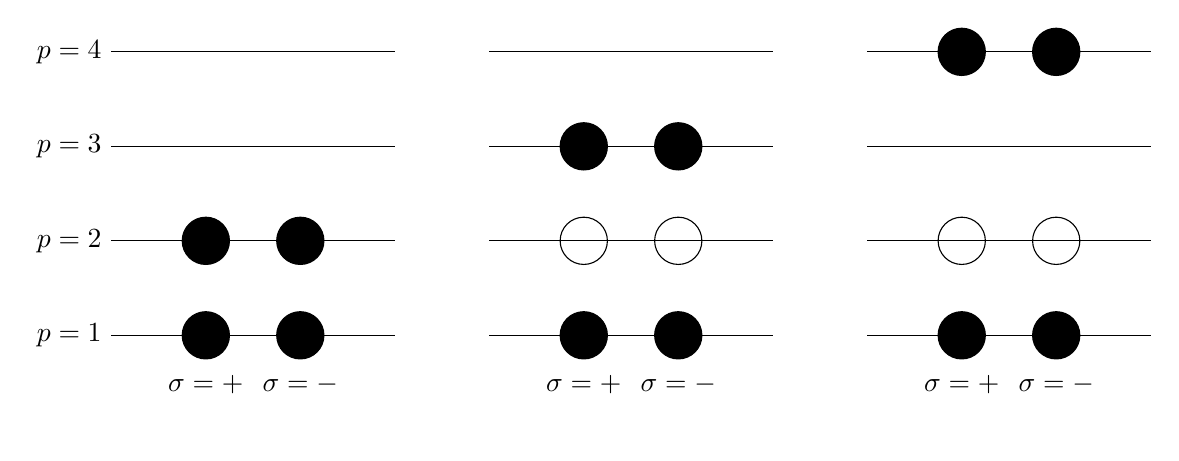
\begin{tikzpicture}[scale=1.2]
		\begin{scope}
		\foreach \i in {1,...,4}
		{
			\draw (-1,\i-1) node[anchor=east] {$p = \i$} --(2,\i-1);
		}
		\filldraw (0,0) node[anchor=north,inner sep=.5cm] {$\sigma=+$} circle (0.25cm); 
		\filldraw (1,0) node[anchor=north,inner sep=.5cm] {$\sigma=-$} circle (0.25cm);
		\filldraw (0,1) circle (0.25cm); 
		\filldraw (1,1) circle (0.25cm);
		\end{scope}
		\begin{scope}[xshift=4cm]
		\foreach \i in {1,...,4}
		{
			\draw (-1,\i-1) --(2,\i-1);
		}
		\filldraw (0,0) node[anchor=north,inner sep=.5cm] {$\sigma=+$} circle (0.25cm); 
		\filldraw (1,0) node[anchor=north,inner sep=.5cm] {$\sigma=-$} circle (0.25cm);
		\draw (0,1) circle (0.25cm); 
		\draw (1,1) circle (0.25cm);
		\filldraw (0,2) circle (0.25cm); 
		\filldraw (1,2) circle (0.25cm);
		\end{scope}
		\begin{scope}[xshift=8cm]
		\foreach \i in {1,...,4}
		{
			\draw (-1,\i-1) --(2,\i-1);
		}
		\filldraw (0,0) node[anchor=north,inner sep=.5cm] {$\sigma=+$} circle (0.25cm); 
		\filldraw (1,0) node[anchor=north,inner sep=.5cm] {$\sigma=-$} circle (0.25cm);
		\draw (0,1) circle (0.25cm); 
		\draw (1,1) circle (0.25cm);
		\filldraw (0,3) circle (0.25cm); 
		\filldraw (1,3) circle (0.25cm);
		\end{scope}
		\end{tikzpicture}
		\newline
		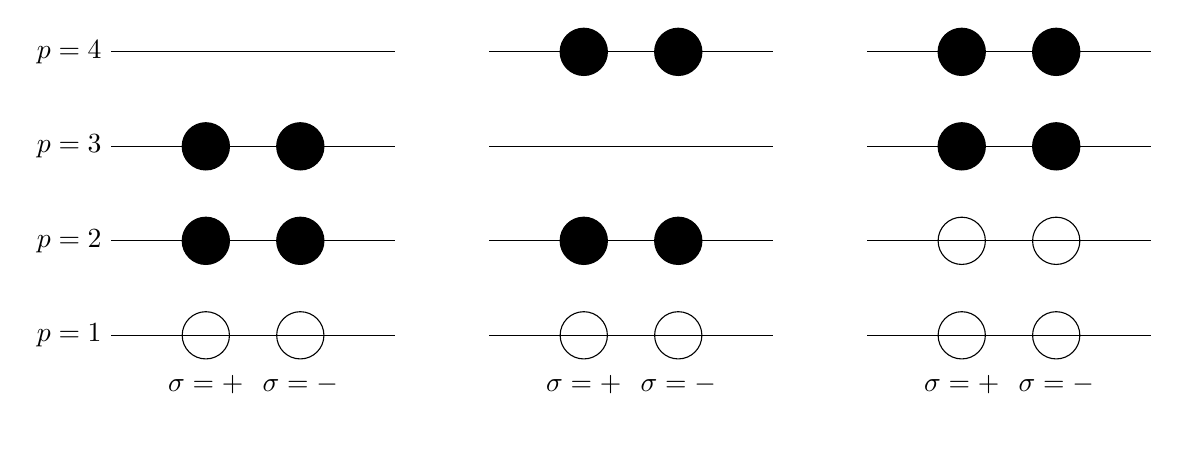
\begin{tikzpicture}[scale=1.2]
		\begin{scope}
		\foreach \i in {1,...,4}
		{
			\draw (-1,\i-1) node[anchor=east] {$p = \i$} --(2,\i-1);
		}
		\draw (0,0) node[anchor=north,inner sep=.5cm] {$\sigma=+$} circle (0.25cm); 
		\draw (1,0) node[anchor=north,inner sep=.5cm] {$\sigma=-$} circle (0.25cm);
		\filldraw (0,1) circle (0.25cm); 
		\filldraw (1,1) circle (0.25cm);
		\filldraw (0,2) circle (0.25cm); 
		\filldraw (1,2) circle (0.25cm);
		\end{scope}
		\begin{scope}[xshift=4cm]
		\foreach \i in {1,...,4}
		{
			\draw (-1,\i-1) --(2,\i-1);
		}
		\draw (0,0) node[anchor=north,inner sep=.5cm] {$\sigma=+$} circle (0.25cm); 
		\draw (1,0) node[anchor=north,inner sep=.5cm] {$\sigma=-$} circle (0.25cm);
		\filldraw (0,1) circle (0.25cm); 
		\filldraw (1,1) circle (0.25cm);
		\filldraw (0,3) circle (0.25cm); 
		\filldraw (1,3) circle (0.25cm);
		\end{scope}
		\begin{scope}[xshift=8cm]
		\foreach \i in {1,...,4}
		{
			\draw (-1,\i-1) --(2,\i-1);
		}
		\draw (0,0) node[anchor=north,inner sep=.5cm] {$\sigma=+$} circle (0.25cm); 
		\draw (1,0) node[anchor=north,inner sep=.5cm] {$\sigma=-$} circle (0.25cm);
		\draw (0,1) circle (0.25cm); 
		\draw (1,1) circle (0.25cm);
		\filldraw (0,2) circle (0.25cm); 
		\filldraw (1,2) circle (0.25cm);
		\filldraw (0,3) circle (0.25cm); 
		\filldraw (1,3) circle (0.25cm);
		\end{scope}
		\end{tikzpicture}
	\end{center}
	\caption{Above all basis states of our pair interaction system are presented schematically with $P=2$ as the number of pairs and $S_z=0$ are the total spin. The solid dots indicate occupied states, while the empty dots indicate unoccupied states (holes). The reference state $|\Phi\rangle$ is represented in the upper left corner. This is all possible states since the excusion principle does not allow two particles with same spin to stay at the same level. For further description, see the text.\label{fig:schematic}}
\end{figure}